\subsection{Experimental Procedure}

For this study, an experiment is a multi-node HPL task run in the same compute allocation with an IOR task of various sizes. These tasks are placed on non-overlapping sets of nodes, creating a situation without any explicit CPU contention. By measuring the HPL completion time of each configuration, we will be able to detect significant runtime impacts.

Figure~\ref{fig:process-layout} demonstrates how tasks are laid out in an allocation. From this basic structure, we created a set of five experiment classes to measure different phenomenon.
\begin{itemize}
\item {\bf HPL-Only:} $k=0,m=0$. This is the control experiment that excludes IOR as a factor. Since this shared experimental infrastructure, BeeOND daemons were configured and started, but the only task running in the compute allocation is an $n$-node HPL job.
\item {\bf Matching Lustre:} $k=0,m=n$. This can be considered another type of control experiment that excludes BeeOND as a factor, while still allowing IOR to potentially demonstrate an impact. This is valuable to determine whether the file system traffic from IOR can perturb an HPL running on other allocated nodes. Crucially, this is the only configuration that does not load any BeeOND daemons.
\item {\bf Single BeeOND:} $k=0,m=1$. This demonstrates the impact of including a single node running a data-intensive workload. 
\item {\bf Matching BeeOND:} $k=0,m=n$. This demonstrates the impact of a larger number of data-intensive processes on HPL performance.
\item {\bf Matching BeeOND (no meta):} $k=1,m=n$. This demonstrates the same type of potential impact as the Matching BeeOND test, but explicitly places a separate task on the same node as the metadata server. This allows us to ensure that the multi-node HPL is not colocated with the metadata server or other management servers we place alongside it. Therefore, the multi-node HPL will only experience performance impacts from the object storage server.
\end{itemize}

\begin{figure}[htbp]
\centerline{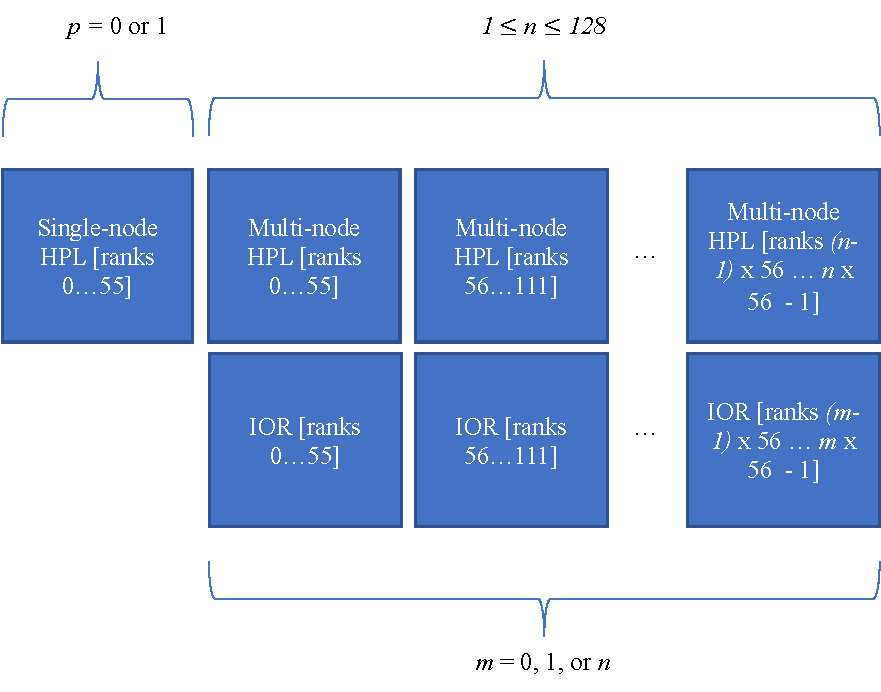
\includegraphics[width=\columnwidth]{process-layout}}
\caption{An illustration demonstrating possible configurations of the experiment.}
\label{fig:process-layout}
\end{figure}

\subsubsection{HPL}
We used HPL~\cite{hpl} as a well-defined compute task to measure. We specified the sizes by starting from a well-performing single-node specification that uses most of the memory on a single node (128MB). When run alone, this takes less than 15 minutes to complete. We then extrapolated to higher node counts by approximating the same amount of work, thus approximately preserving the total runtime of each experiment. This means that, while runs of the same node count are comparable, runs of different node counts are not directly comparable. The problem sizes we used are in Table~\ref{tab:hpl-params}. %We were reminded that Q should be larger than P (\url{https://icl.utk.edu/hpcc/faq/index.html#124}), but we do not believe that this causes any issues with our measurements.


\begin{table}[htbp]
\caption{HPL Parameters by Node Count}
\begin{center}
\begin{tabular}{|c|c|c|c|}
\hline
\textbf{Node Count}&\textbf{Row Count (N)} & \textbf{Grid P} & \textbf{Grid Q} \\
\hline
1 & 91048 & 7 & 8 \\
2 & 114713 & 14 & 8 \\
4 & 144529 & 14 & 16 \\
8 & 182096 & 28 & 16 \\
16 & 229427 & 28 & 32 \\
32 & 289059 & 56 & 32 \\
64 & 364192 & 56 & 64 \\
128 & 458853 & 112 & 64 \\
%256 & 578119 & 112 & 128 \\
\hline
\end{tabular}
\label{tab:hpl-params}
\end{center}
\end{table}

\subsubsection{IOR}
We used IOR to approximate a data-intensive write task. We designed the IOR task to be as disruptive to object storage daemons as possible by having it create many small synchronous writes from as many processes as possible throughout the runtime of the compute tasks. Since the I/O tasks are designed to run through the entire compute task, we structured the IOR job so that it would not reasonably terminate during the computation. Once the computation was complete, the IOR task was killed. Table~\ref{tab:ior-params} describes the specific options we used for IOR.

\begin{table}[htbp]
\caption{IOR Parameters}
\begin{center}
\begin{tabular}{|c|c|c|}
  \hline
  \textbf{Parameter} & \textbf{Description} & \textbf{Value} \\
%\textbf{Node Count}&\textbf{Row Count (N)} & \textbf{Grid P} & \textbf{Grid Q} \\
  \hline
      [srun] -n & Processes (per node) & 56 \\
      -t & Transfer size (bytes) & 512 \\
      -T & Maximum run duration (minutes) & 20 \\
      -D & Stonewalling deadline (seconds) & 60 \\
      -i & Test repetitions & 1048576 \\
      -e & Sync after each write phase & enabled \\
      -C & Reorder tasks & enabled \\
      -w & Perform write test & enabled \\
      -a & Access method & POSIX \\
      -s & Number of segments & 1024 \\
      -F & Use file-per-process & enabled \\
      -Y & Sync after every write & enabled \\      
\hline
\end{tabular}
\label{tab:ior-params}
\end{center}
\end{table}




